\documentclass[tikz,border=2pt]{standalone}
\usepackage{pgfplots}
\usetikzlibrary{intersections}
\usepgfplotslibrary{fillbetween}
\pgfplotsset{compat=1.7}

\begin{document}
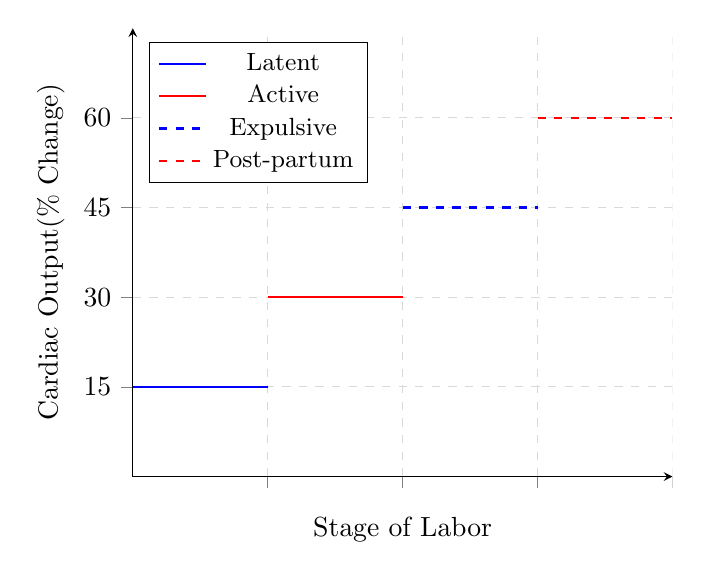
\begin{tikzpicture}


\begin{axis}[
        axis lines=middle,
        grid = major,
        grid style={dashed, gray!30},
	ymin = 0,
	ymax = 75,
	xmin = 0,
	xmax =4,
	 ylabel near ticks,
	xlabel near ticks,
        xlabel=Stage of Labor,
        ylabel=Cardiac Output \\ (\% Change),
        tick align=outside,
        enlargelimits=false,
ytick={15,30, 45, 60},
yticklabels = {15, 30, 45, 60},
xticklabels = {\empty}
ylabel style={align=center},
legend pos= north west,
legend style={font=\small, cells={align=left}}]

\addplot[blue,thick, domain=0:1] {15};
\addlegendentry{Latent};
\addplot[red,thick, domain=1:2] {30};
\addlegendentry{Active};
\addplot[blue,dashed, thick, domain=2:3] {45};
\addlegendentry{Expulsive};
\addplot[red,dashed, thick, domain=3:4] {60};
\addlegendentry{Post-partum};

\end{axis}

\end{tikzpicture} 
\end{document}